\documentclass[12pt]{article}
\usepackage[utf8]{inputenc}
\usepackage[czech]{babel}
\usepackage[a4paper, top=2cm, bottom=2cm, left=2cm, right=2cm]{geometry}
\usepackage[IL2]{fontenc}
\usepackage{url}
\usepackage{indentfirst}
\usepackage{amsthm}
\usepackage{amsmath}
\usepackage{graphicx}
\usepackage{listings}
\usepackage{color}
\usepackage{subfig}
\usepackage{float}
\usepackage{multirow}
\usepackage{booktabs}
\usepackage[table,usenames,dvipsnames,svgnames]{xcolor}
\usepackage[unicode,hyperindex,plainpages=false,pdftex]{hyperref}
\usepackage{algpseudocode}   
    \hypersetup{
          colorlinks=true, 
          linkcolor=BrickRed, 
          citecolor=OliveGreen, 
          filecolor=magenta, 
          urlcolor=cyan
    }


\newcommand{\todo}[1]{\textcolor{red}{[[TODO: #1]]}}

\newlength{\skipeqarray}
\setlength{\skipeqarray}{0.4cm}

\title{Algoritmus pro hledání maximálních nezávislých množin}
\author{Milan Munzar\\
Jakub Sochor\\
\normalsize{\url{xmunza00}, \url{xsocho06} }}
\date{}

\definecolor{lightgray}{rgb}{0.9, 0.9, 0.9}

\newtheorem{veta}{Věta}
\newtheorem{priklad}{Příklad}
\newfloat{algorithm}{h}{lop}
\floatname{algorithm}{Algoritmus}

\renewcommand{\algorithmicrequire}{\textbf{Vstup:}}
\renewcommand{\algorithmicensure}{\textbf{Výstup:}}
\renewcommand{\algorithmiccomment}[1]{// #1}

\begin{document}
\maketitle

\section{Úvod}



\section{Maximální nezávislé množiny}

Množina vrcholů grafu je nezávilá, když žádné dva vrcholy v této množině nejsou spojeny hranou. Tato množina je maximální, pokud k ní už nelze přidat žádný vrchol a zároveń dodržet podmínku nezávislosti.

\todo{formálně}

Typickou úlohou pro nalezení nezávislých množin je hledání prvků, které spolu mohou nějakým způsobem fungovat. Mohou to být například procesy počítače, jež pracují nad společnými daty. Procesy jsou tomto případě vrcholy grafu a budou spojeny hranou v případě, že pro svůj běh potřebují stejná data. Nezávislá množina potom bude obsahovat ty procesy, které mohou běžet současně.

Hledání maximálních nezávislých množin je NP-těžšký problém. Jedinou známou možností jak tento problém řešit je procházet všechny podmnožiny množiny vrcholů a určovat zda je zvolená množina maximální nezávislá. Jelikož množství podmnožin roste exponenciálně s počtem vrcholů je toto řešení pro velké grafy náročné.

Často se v aplikacích  setkáváme s potřebou určit nezávislost grafu. Nezávislost grafu \(G\) je rovna velikosti nejpočetnější nezávislé množiny a značí se \(\alpha(G)\). Tato množina je zároveń množinou maximální, ale naopak to neplatí. Jiným požadavkem může být například nalezení nejdražší nezávislé množiny ve smyslu ohodnocení vrcholů.

Pojmy úzce související s maximálními nezávislými množinami jsou klika grafu a dominující podmnožina. Klika je maximální úplný podgraf grafu \(G\) a odpovídá nějaké maximální nezavislé množině doplńkového grafu \(-G\). Dominující podmnožina vrcholů grafu jsou ty vrcholy, jež se svými sousedy pokrávají celý graf. Tedy každá maximální nezávislá množina je zároveń množinou dominující.

\subsection{Popis použitého algoritmu}
Implementovaný algoritmus jsme převzali z \cite{demel}. Jeho základem je metoda zpětného navracení. Složitost je \(O(2^{n/3})\) \todo{Zkontrolovat složitost}, kde \(n\) je počet uzlů grafu \cite{tarjan}. Algoritmus lze upravit pro hledání nejpočetnější nebo nejdražší nezávislé množiny. Během svého běhu si udržuje 3 navzájem disjunktní množiny vrcholů \(R, N, S\). \(R\) je nezávislá množina vrcholů. Množina \(N\) obsahuje vrcholy, které nebyli přidány \(R\). \(S\) obsahuje vrcholy, které již tvořily maximální nezávislou množinu.

\begin{algorithm}
\caption{Hledání maximálních nezávislých množin}
\begin{algorithmic}

\While{1}
                          
  \If {$N_k \neq \emptyset \lor S_K \neq \emptyset$}
    \If{$N_k \neq \emptyset$}
      \If{$ \exists y : V(y) \cap S_k \neq \emptyset $}
        \State{reduce $\leftarrow$ FALSE}
      \EndIf    
    \EndIf
  \EndIf
  
  \Comment{Rozšíření nebo zkrácení nezávislé množiny}
  \If {reduce = FALSE}
    \State $k \leftarrow k+1$
    \State $R \leftarrow \{x\} \in N$
  \Else
  
  \EndIf


\EndWhile 
\end{algorithmic}
\end{algorithm}

Jiným řešením pro nalezení maximálních nezávislých množin je například Robsonův algoritmus se složitostí \(O(2^{0.296n})\) \cite{robson}. Fomin dosáhl složitosti \(O(2^{0.288n})\) pomocí metody rozděl a panuj \cite{fomin}. Tyto algoritmy využívají heuristiky pro vyloučení některých množin z prohledávání a pro výběr uzlu.  

\section{Implementace}
Úprava algoritmu pro paralelizaci, využité prostředky pro paralelizaci~\ref{appendix:ProgramUsage}


\section{Vyhodnocení}
Pro účely vyhodnocení zrychlení paralelní verze algoritmu oproti sekvenční byly vytvořeny skripty, které generují náhodné grafy se zadaným počtem vrcholů a~hran ve formátu GraphML. 

Jednotlivé grafy jsou rozděleny do skupin podle toho, kolik procent maximálního možného počtu hran obsahují. K~tomuto rozdělení jsme přistoupili zejména proto, aby čas běhu algoritmu v~jedné skupině grafů byl rostoucí s~počtem vrcholů daného zpracovávaného grafu, jelikož počet hran grafu významně ovlivňuje také počet maximálních nezávislých množin v~daném grafu a~tudíž i~dobu běhu. 

Celé vyhodnocování bylo prováděno na třech skupinách grafů po 31 grafech ve skupině. Program byl vždy puštěn sekvenčně a~změřen čas běhu $t_S$ a~následně byl puštěn paralelně a~určen čas $t_P$, po který pracovala paralelní verze algoritmu. Do změřených časů není započteno načítání grafu ani případný výpis maximálních nezávislých množin, ale pouze čistý čas běhu algoritmu pro určení těchto množin. Pro každý graf bylo určeno zrychlení $s$ podle vzorce~\ref{eq:Speedup}.
\begin{equation}
    s = \frac{t_S}{t_P} \label{eq:Speedup}
\end{equation}

Testování bylo prováděno na počítači s procesorem AMD Phenom X4 945, který má 4 fyzická jádra běžící na frekvenci 3\,GHz a~4\,GB RAM. Během běhu programu nebyl na počítači puštěn žádný další výpočetně náročný proces a~pro měření času bylo využito \texttt{high\_resolution\_clock} ze standardu C++11. \todo{přidat přesnost???}

Grafy vytvořené z~naměřených výsledků lze vidět na obrázku~\ref{fig:SpeedResults} a~všechny naměřené časy a~určené zrychlení jsou obsaženy v~příloze~\ref{appendix:RawResults}.

\begin{figure}[p]
    \centering
    \subfloat[$50\,\%$ hran]{ 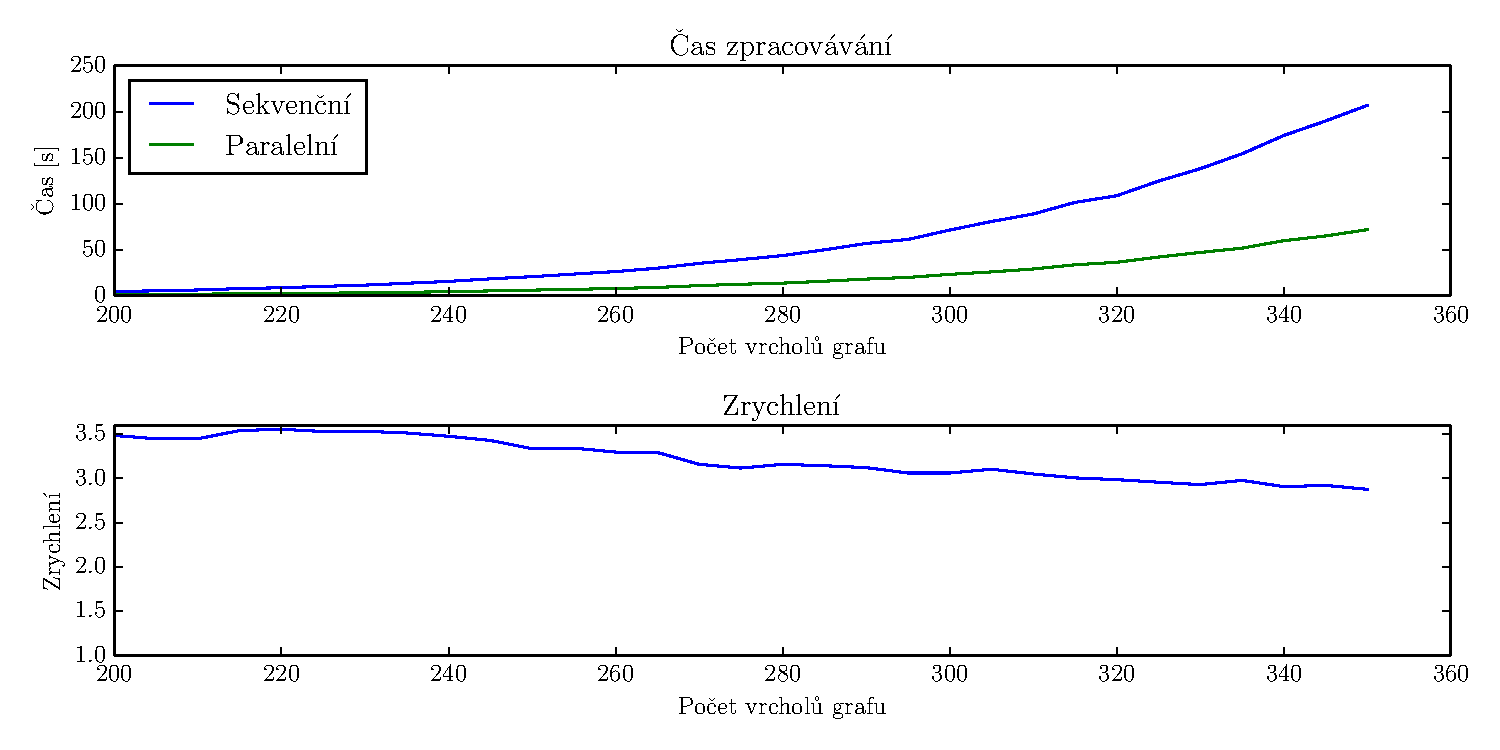
\includegraphics[scale=0.55]{images/5.pdf}}\\
    \subfloat[$60\,\%$ hran]{ 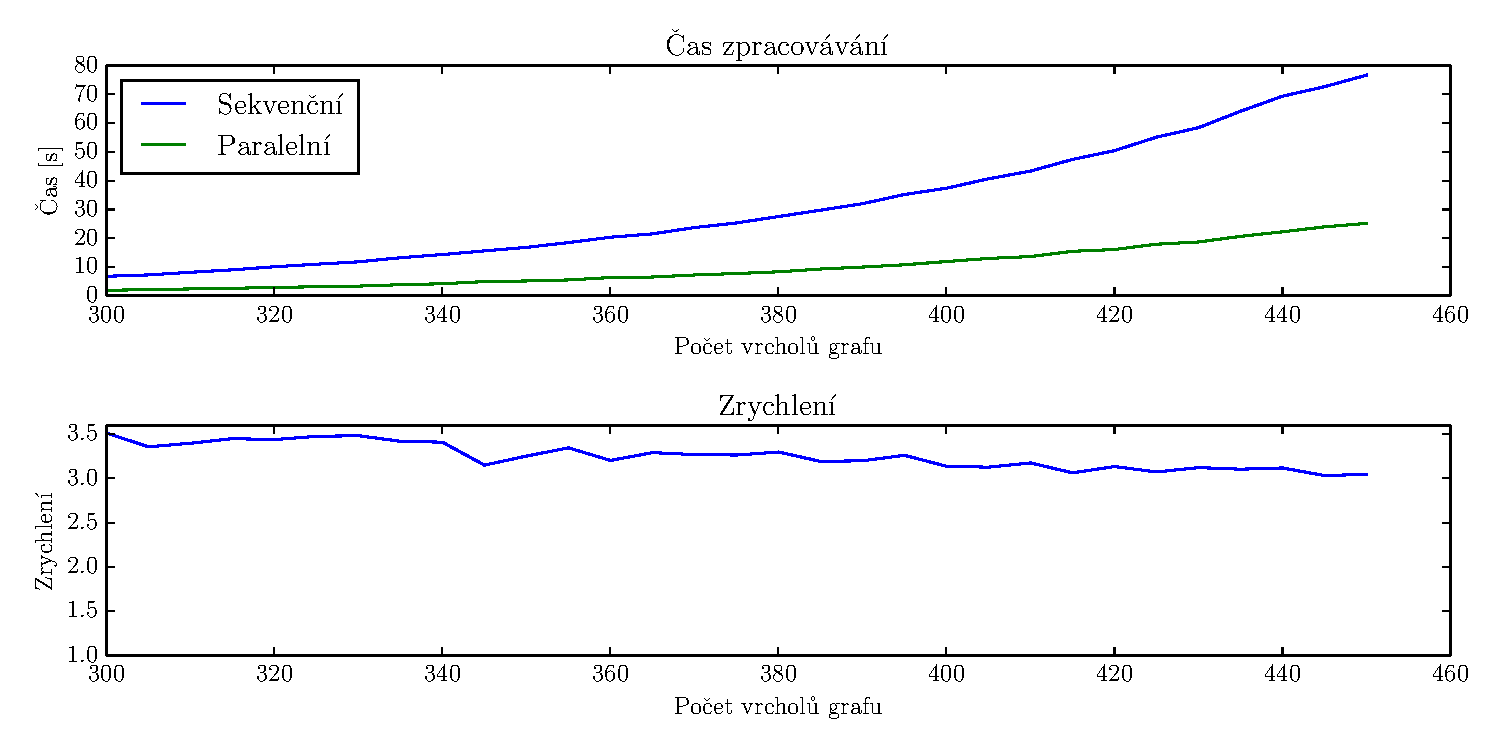
\includegraphics[scale=0.55]{images/6.pdf}}\\
    \subfloat[$70\,\%$ hran]{ 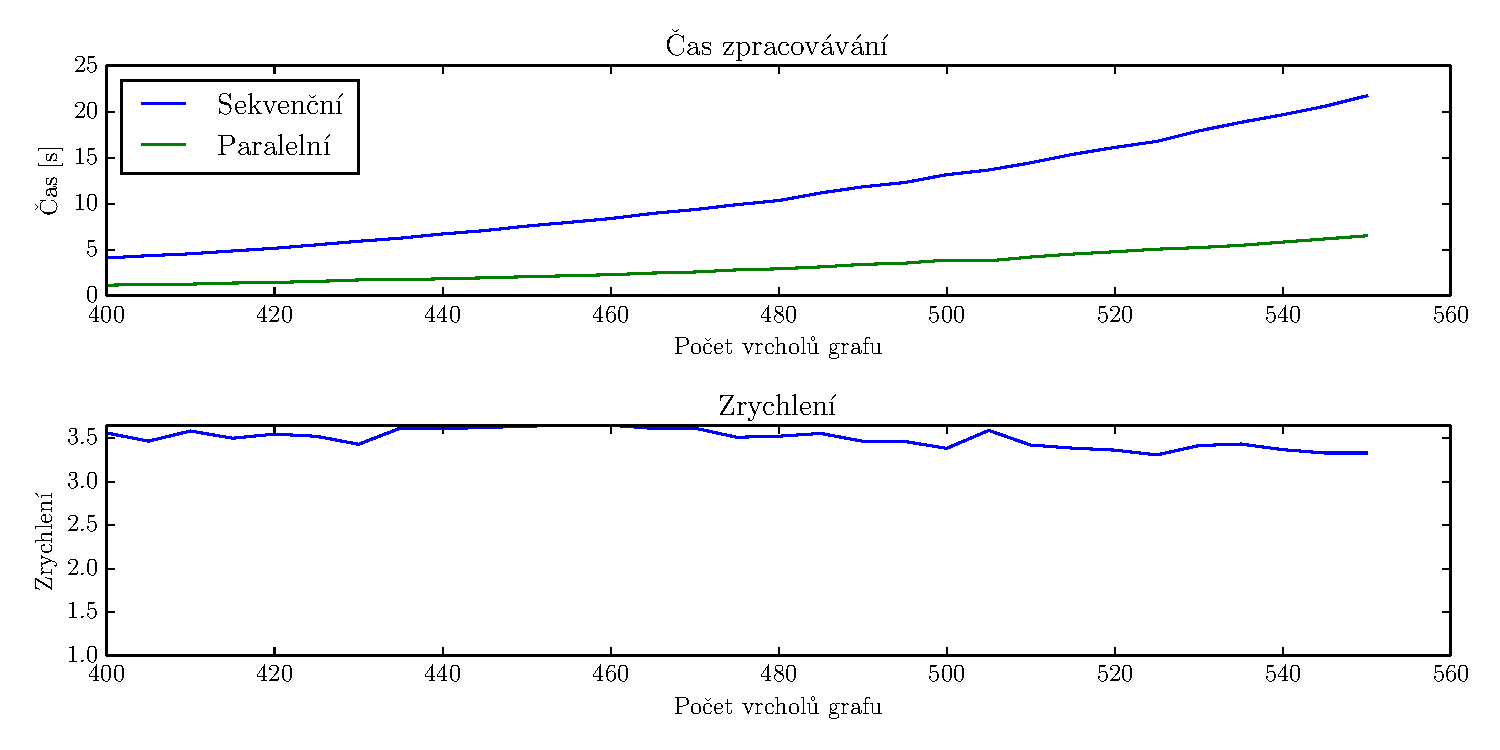
\includegraphics[scale=0.55]{images/7.pdf}}
    \caption{Naměřené výsledky rychlosti hledání maximálních nezávislých množin a~zrychlení oproti sekvenčnímu algoritmu. Grafy obsažené v~jednom grafu obsahují stejné procento všech hran.} \label{fig:SpeedResults}
\end{figure}


Maximální teoreticky možné dosažitelné zrychlení na procesoru se čtyřmi jádry je 4,0. Jak lze vidět z~uvedených grafů, tak nám se podařilo dosáhnout zrychlení kolem 3,5. Toto považujeme za solidní výsledek, protože v~rámci programu je též nutné řešit synchronizaci přístupu do struktury obsahující výsledné maximální nezávislé množiny. 

Ovšem jak si lze z~grafů všimnout, tak s~narůstajícím počtem vrcholů se zrychlení snižuje. Tento fakt je dle našeho zkoumání způsoben především tím, že velmi zásadně roste počet maximálních nezávislých množin a~jejich reprezentace v~paměti již není triviální a~program celkově využije velkého množství paměti (více než 1\,GB). 

Kvůli tomuto problému jsme také experimentovali s~tím, že se maximální nezávislé množiny nebudou ukládat do paměti, ale rovnou vypisovat. S~tímto přístupem jsme ovšem dosahovali ještě horších výsledků, jelikož program trávil podstatně další čas v~kritické sekci výpisu výsledku a~tímto byla paralelní verze programu velmi zpomalena. 

\section{Závěr}

\begin{thebibliography}{99}

\bibitem{demel} 
    DEMEL, Jiří. \emph{Grafy a jejich aplikace}. Vyd. 1. Praha: Academia, 2002, 257 s. ISBN 80-200-0990-6.

\bibitem{robson}
ROBSON, J.M. \emph{Algorithms for maximum independent sets}. Journal of Algorithms. 1986, vol. 7, issue 3, s. 425-440.

\bibitem{fomin}
  FOMIN, Fedor V., FABRIZIO Grandoni, DIETER Kratsch.
  \emph{Measure and conquer: a simple O($2^{0.288n}$) independent set algorithm}.
  Proceedings of the seventeenth annual ACM-SIAM symposium on Discrete algorithm.
   ACM, 2006.

\bibitem{tarjan}
  TARJAN, Robert Endre, TROJANOWSKI Anthony E.
  \emph{Finding a maximum independent set.}
  SIAM Journal on Computing 6.3 (1977): 537-546.

\end{thebibliography}

\appendix
\section{Použití programu} \label{appendix:ProgramUsage}

\section{Naměřené výsledky} \label{appendix:RawResults}

\begin{table}[H]
\begin{center}
\rowcolors{2}{lightgray}{white}
\begin{tabular}{ c c c c c }
\toprule
Vrcholů & Hran & Sekvenční [s] & Parelelní [s] & Zrychlení\\\midrule
200 & 9950 & 4.806 & 1.379 & 3.484\\
205 & 10455 & 5.457 & 1.583 & 3.446\\
210 & 10972 & 6.417 & 1.862 & 3.447\\
215 & 11502 & 7.905 & 2.233 & 3.539\\
220 & 12045 & 8.834 & 2.486 & 3.554\\
225 & 12600 & 10.320 & 2.926 & 3.528\\
230 & 13167 & 11.675 & 3.307 & 3.531\\
235 & 13747 & 13.686 & 3.897 & 3.512\\
240 & 14340 & 15.704 & 4.519 & 3.475\\
245 & 14945 & 18.481 & 5.391 & 3.428\\
250 & 15562 & 20.852 & 6.254 & 3.334\\
255 & 16192 & 23.675 & 7.085 & 3.341\\
260 & 16835 & 26.377 & 8.003 & 3.296\\
265 & 17490 & 30.030 & 9.123 & 3.292\\
270 & 18157 & 35.272 & 11.169 & 3.158\\
275 & 18837 & 39.345 & 12.627 & 3.116\\
280 & 19530 & 43.736 & 13.849 & 3.158\\
285 & 20235 & 49.988 & 15.907 & 3.142\\
290 & 20952 & 56.912 & 18.233 & 3.121\\
295 & 21682 & 61.219 & 20.003 & 3.060\\
300 & 22425 & 71.425 & 23.343 & 3.060\\
305 & 23180 & 80.738 & 26.021 & 3.103\\
310 & 23947 & 88.890 & 29.152 & 3.049\\
315 & 24727 & 101.445 & 33.761 & 3.005\\
320 & 25520 & 108.687 & 36.410 & 2.985\\
325 & 26325 & 124.581 & 42.150 & 2.956\\
330 & 27142 & 138.036 & 47.123 & 2.929\\
335 & 27972 & 154.214 & 51.808 & 2.977\\
340 & 28815 & 174.083 & 59.911 & 2.906\\
345 & 29670 & 189.836 & 65.013 & 2.920\\
350 & 30537 & 206.761 & 71.886 & 2.876\\
\bottomrule
\end{tabular}
\end{center}
\caption{Naměřené výsledky pro grafy s~$50\,\%$ hran} 
\end{table}

\begin{table}[H]
\begin{center}
\rowcolors{2}{lightgray}{white}
\begin{tabular}{ c c c c c }
\toprule
Vrcholů & Hran & Sekvenční [s] & Parelelní [s] & Zrychlení\\\midrule
300 & 26910 & 6.805 & 1.938 & 3.511\\
305 & 27816 & 7.280 & 2.169 & 3.356\\
310 & 28737 & 8.192 & 2.413 & 3.396\\
315 & 29673 & 9.049 & 2.624 & 3.448\\
320 & 30624 & 10.111 & 2.942 & 3.437\\
325 & 31590 & 11.002 & 3.167 & 3.474\\
330 & 32571 & 11.819 & 3.395 & 3.481\\
335 & 33567 & 13.254 & 3.878 & 3.418\\
340 & 34578 & 14.360 & 4.213 & 3.408\\
345 & 35604 & 15.617 & 4.960 & 3.149\\
350 & 36645 & 16.846 & 5.182 & 3.251\\
355 & 37701 & 18.513 & 5.536 & 3.344\\
360 & 38772 & 20.369 & 6.360 & 3.202\\
365 & 39858 & 21.536 & 6.546 & 3.290\\
370 & 40959 & 23.727 & 7.260 & 3.268\\
375 & 42075 & 25.338 & 7.765 & 3.263\\
380 & 43206 & 27.552 & 8.358 & 3.297\\
385 & 44352 & 29.760 & 9.326 & 3.191\\
390 & 45513 & 32.013 & 10.009 & 3.198\\
395 & 46689 & 35.218 & 10.803 & 3.260\\
400 & 47880 & 37.397 & 11.926 & 3.136\\
405 & 49086 & 40.661 & 13.008 & 3.126\\
410 & 50307 & 43.336 & 13.655 & 3.174\\
415 & 51543 & 47.390 & 15.475 & 3.062\\
420 & 52794 & 50.443 & 16.103 & 3.133\\
425 & 54060 & 55.128 & 17.948 & 3.072\\
430 & 55341 & 58.416 & 18.720 & 3.121\\
435 & 56637 & 64.123 & 20.668 & 3.103\\
440 & 57948 & 69.349 & 22.250 & 3.117\\
445 & 59274 & 72.653 & 23.972 & 3.031\\
450 & 60615 & 76.661 & 25.176 & 3.045\\
\bottomrule
\end{tabular}
\end{center}
\caption{Naměřené výsledky pro grafy s~$60\,\%$ hran} 
\end{table}

\begin{table}[H]
\begin{center}
\rowcolors{2}{lightgray}{white}
\begin{tabular}{ c c c c c }
\toprule
Vrcholů & Hran & Sekvenční [s] & Parelelní [s] & Zrychlení\\\midrule
400 & 55860 & 4.118 & 1.156 & 3.561\\
405 & 57267 & 4.361 & 1.258 & 3.466\\
410 & 58691 & 4.567 & 1.275 & 3.583\\
415 & 60133 & 4.875 & 1.393 & 3.500\\
420 & 61592 & 5.169 & 1.457 & 3.547\\
425 & 63069 & 5.538 & 1.572 & 3.522\\
430 & 64564 & 5.929 & 1.729 & 3.430\\
435 & 66076 & 6.263 & 1.731 & 3.617\\
440 & 67606 & 6.720 & 1.862 & 3.610\\
445 & 69153 & 7.085 & 1.956 & 3.623\\
450 & 70717 & 7.570 & 2.081 & 3.638\\
455 & 72299 & 7.977 & 2.185 & 3.650\\
460 & 73899 & 8.391 & 2.299 & 3.650\\
465 & 75516 & 8.952 & 2.478 & 3.613\\
470 & 77150 & 9.362 & 2.589 & 3.616\\
475 & 78802 & 9.900 & 2.819 & 3.511\\
480 & 80472 & 10.345 & 2.936 & 3.523\\
485 & 82159 & 11.172 & 3.143 & 3.555\\
490 & 83863 & 11.838 & 3.417 & 3.465\\
495 & 85585 & 12.301 & 3.552 & 3.463\\
500 & 87325 & 13.155 & 3.888 & 3.383\\
505 & 89082 & 13.664 & 3.806 & 3.590\\
510 & 90856 & 14.445 & 4.222 & 3.421\\
515 & 92648 & 15.364 & 4.538 & 3.386\\
520 & 94458 & 16.111 & 4.790 & 3.363\\
525 & 96285 & 16.770 & 5.069 & 3.308\\
530 & 98129 & 17.903 & 5.243 & 3.415\\
535 & 99991 & 18.835 & 5.486 & 3.433\\
540 & 101871 & 19.660 & 5.838 & 3.368\\
545 & 103768 & 20.578 & 6.180 & 3.330\\
550 & 105682 & 21.710 & 6.519 & 3.330\\
\bottomrule
\end{tabular}
\end{center}
\caption{Naměřené výsledky pro grafy s~$70\,\%$ hran} 
\end{table}

\end{document}
